\section{System Modelling}
\label{ch4:sec:system-modelling}

In this section, Section \ref{ch4:sec:system-modelling} the underlying assumptions to validate the research are presented.
Then the EV charging model and a BESS model are explained.
In the end of this section, the network models that are used to simulate the power distribution networks are presented.

\subsection{Assumptions}
\label{ch4:subsec:assumptions}

Several underlying assumption were made to obtain the models that are used throughout this work :

\begin{enumerate}
\item
The uptake of EVs is assumed to increase and, hence, to have a significant impact on the normal operation of the low voltage distribution network.
This assumption is based on a well-established prediction that the majority of EV charging will take place at home \cite{Munkhammar2015a}.
\item
The transition from internal combustion engine-powered vehicles to EVs is assumed to not impact the users' driving behaviour - apart from the introduction of home-charging.
Similar to \cite{Dallinger2012} this assumption allows the utilisation of recent vehicle mobility data \cite{MiD2008} to generate leaving, driving and arriving probabilities, from which the EV charging demand can be determined and the resulting energy demand can be calculated.
\item
The transition to low carbon technologies will increase the variability of electricity demand and therefore, grid-supporting devices such as BESS are anticipated to play a more important role \cite{FES2015}.
Hence, alongside a high uptake of EVs an increased adoption of distributed BESS devices is assumed.
\item
A realistic behaviour of BESS is also assumed since they are not 100\% efficient at storing and releasing electrical energy as in \cite{Rowe2014a}.
Furthermore the assumption is made that BESS start the simulations at 50\% State of Charge (SOC).
Additionally, it is assumed that BESS utilisation will degrade its energy storage capability and power performance over time as shown in \cite{Laresgoiti2015}.
Therefore, the requirements for equal and fair storage usage is of high importance.
\item
It is assumed that the load profiles provided by the IEEE Power and Energy Society (PES) are sufficient as base load profiles for all simulations and capture enough realistic demand variability to generate results from which conclusions (regarding the algorithm performance) can be drawn.
\end{enumerate}

\subsection{EV charging behaviour}
\label{ch4:subsec:ev-charging-behaviour}

\nomenclature[L]{$n_{s}(t)$}{Probability of starting a trip, where $n_{s}(t) \in [0, 1]$}
\nomenclature[L]{$w_{x}(t)$}{Trip distance probability for weekends ($w_{we}(t)$) and week-days ($w_{wd}(d)$), where $w_{x}(t) \in [0, 1]$}
\nomenclature[L]{$\hat{n}_x(t)$}{Predicted EV demand data, where $n_{r}(t) \in \mathbb{R}$}

An empirical EV model was developed to capture the underlying driving behaviour that was captured in the publicly-available car mobility dataset named \textit{Mobilit\"{a}t in Deutschland} that was published by the German Department of Transport \cite{MiD2008} and validated by Dallinger et al. in \cite{Dallinger2012}.
This dataset contained three parts: the probability of starting a trip, $n_{s}(t)$, the probability of a weekday trip being of a certain distance, $w_{wd}(t)$, and the probability of a weekend trip being of a certain distance, $w_{we}(t)$.
Both probabilities are at a 15 minutely period.
The probability of starting a trip (i.e. $n_{s}(t)$) is approximated by three continuous normal distribution functions since it is assumed that driver behaviour is distributed normally around three key times throughout the day.
\hladd{These three key times are: morning time to leave home to drive to work; lunchtime to leave home to run errands; and evening time to return home.
It should be noted that the naming is purely for exemplification and that this choice of three normal distributions reflects the average vehicle usage determined in the dataset }\cite{MiD2008}\hladd{ although individual driving behaviour may differ from these three events.
Therefore, and to avoid splitting the dataset into an arbitrarily large number of approximating distributions, these three daily events are chosen as a basis for the subsequent work, and }\hlrem{E}\hladd{e}ach distribution is based on the subsequent equation of a normal distribution:

\begin{equation}
\hat{n}_x(t) = \beta_x\frac{1}{\sigma_x\sqrt{2\pi}} \exp\left[-\frac{\left(^t/_{24}-\mu_x\right)^2}{2\sigma_x^2}\right] \;\text{where}\; t = [0, 24]
\label{ch4:equ:normal-distribution}
\end{equation}


For better readability and since they are function specific constants, $\beta_x$, $\mu_x$ and $\sigma_x$ are dropped from the equations within the text - i.e. $\hat{n}_x(\beta_x,\mu_x,\sigma_x,t)$ is abbreviated by $\hat{n}_x(t)$.
From Equation \ref{ch4:equ:normal-distribution} a probability distribution is denoted $\hat{n}_{m}(t)$ to represent the probability of a vehicle leaving in the morning.
$\hat{n}_{l}(t)$ represents the probability of it leaving during lunch time and $\hat{n}_{e}(t)$ represents the probability of an EV leaving during the evening.
If it is assumed that vehicles perform a round trip from their home to a certain location and back, then a symmetric commuting behaviour (i.e. vehicles departing in the morning return during the evening) and an equality amongst the three probabilities (i.e. a constraint) can be defined as follows:

\begin{equation}
0 = \int_{0}^{24}\hat{n}_m(t) + \hat{n}_l(t) - \hat{n}_e(t) dt
\label{ch4:equ:normal-distribution-balance}
\end{equation}


To approximate the original probability of starting a trip, the difference between these three probability functions' aggregate and the original distribution (i.e. $n_s(t)$) had to be minimised.
Therefore, this minimisation problem is defined as follows:

\begin{equation}
\begin{split}
	\min_{\boldsymbol{\beta}, \boldsymbol{\mu}, \boldsymbol{\sigma}}& \int_{0}^{24}\left(\hat{n}_m(\beta_m,\mu_m,\sigma_m,t) + \hat{n}_l(\beta_l,\mu_l,\sigma_l,t) + \hat{n}_e(\beta_e,\mu_e,\sigma_e,t) - n_s(t)\right)^2 dt\\
	\text{s.t.}&
	\begin{cases}
		0 = \int_{0}^{24}\hat{n}_m(\beta_m,\mu,_m\sigma_m,t) + \hat{n}_l(\beta_l,\mu_l,\sigma_l,t) - \hat{n}_e(\beta_e,\mu_e,\sigma_e,t) dt \\
		1 = \int_{0}^{24}\hat{n}_m(\beta_m,\mu_m,\sigma_m,t) dt \\
		1 = \int_{0}^{24}\hat{n}_l(\beta_l,\mu_l,\sigma_l,t) dt \\
		1 = \int_{0}^{24}\hat{n}_e(\beta_e,\mu_e,\sigma_e,t) dt
	\end{cases}\\
	\text{where }& \boldsymbol{\beta} = \{\beta_m, \beta_l, \beta_e\} \text{ and } \boldsymbol{\mu} = \{\mu_m, \mu_l, \mu_e\} \text{ and } \boldsymbol{\sigma}  = \{\sigma_m, \sigma_l, \sigma_e\}
\end{split}
\label{ch6:equ:normal-distribution-minimisation}
\end{equation}

This minimisation problem was solved using a Generalised Reduced Gradient (GRG) algorithm so that the obtained parameters make the three functions fit best to the original dataset.
The resulting parameters from the GRG fitting of the three distribution functions are tabulated in Table~\ref{ch4:tab:starting-a-trip-probability}.
Additionally, the resulting departure probabilities as well as the original data (i.e. $n_s(t)$) are shown in Figure~\ref{ch4:fig:starting-a-trip-probability} for visualisation.

\begin{table}\centering
	\begin{tabular}{cccc}
	\hline
	\textbf{Equation} \boldmath{$\hat{n}_x(t)$} & \boldmath{$\mu_x$} \textbf{(Mean)} & \boldmath{$\sigma_x$} \textbf{(SD)} & \boldmath{$\beta_x$} \textbf{(Weight)} \\
	\hline
	$\hat{n}_m(t)$ & 0.3049 & 0.0488 & 0.00206 \\
	$\hat{n}_l(t)$ & 0.4666 & 0.0829 & 0.00314 \\
	$\hat{n}_e(t)$ & 0.7042 & 0.0970 & 0.00521\\
	\hline
	\end{tabular}
	\caption{Parameters for normal distributions.}
	\label{ch4:tab:starting-a-trip-probability}
\end{table}


\begin{figure}\centering
	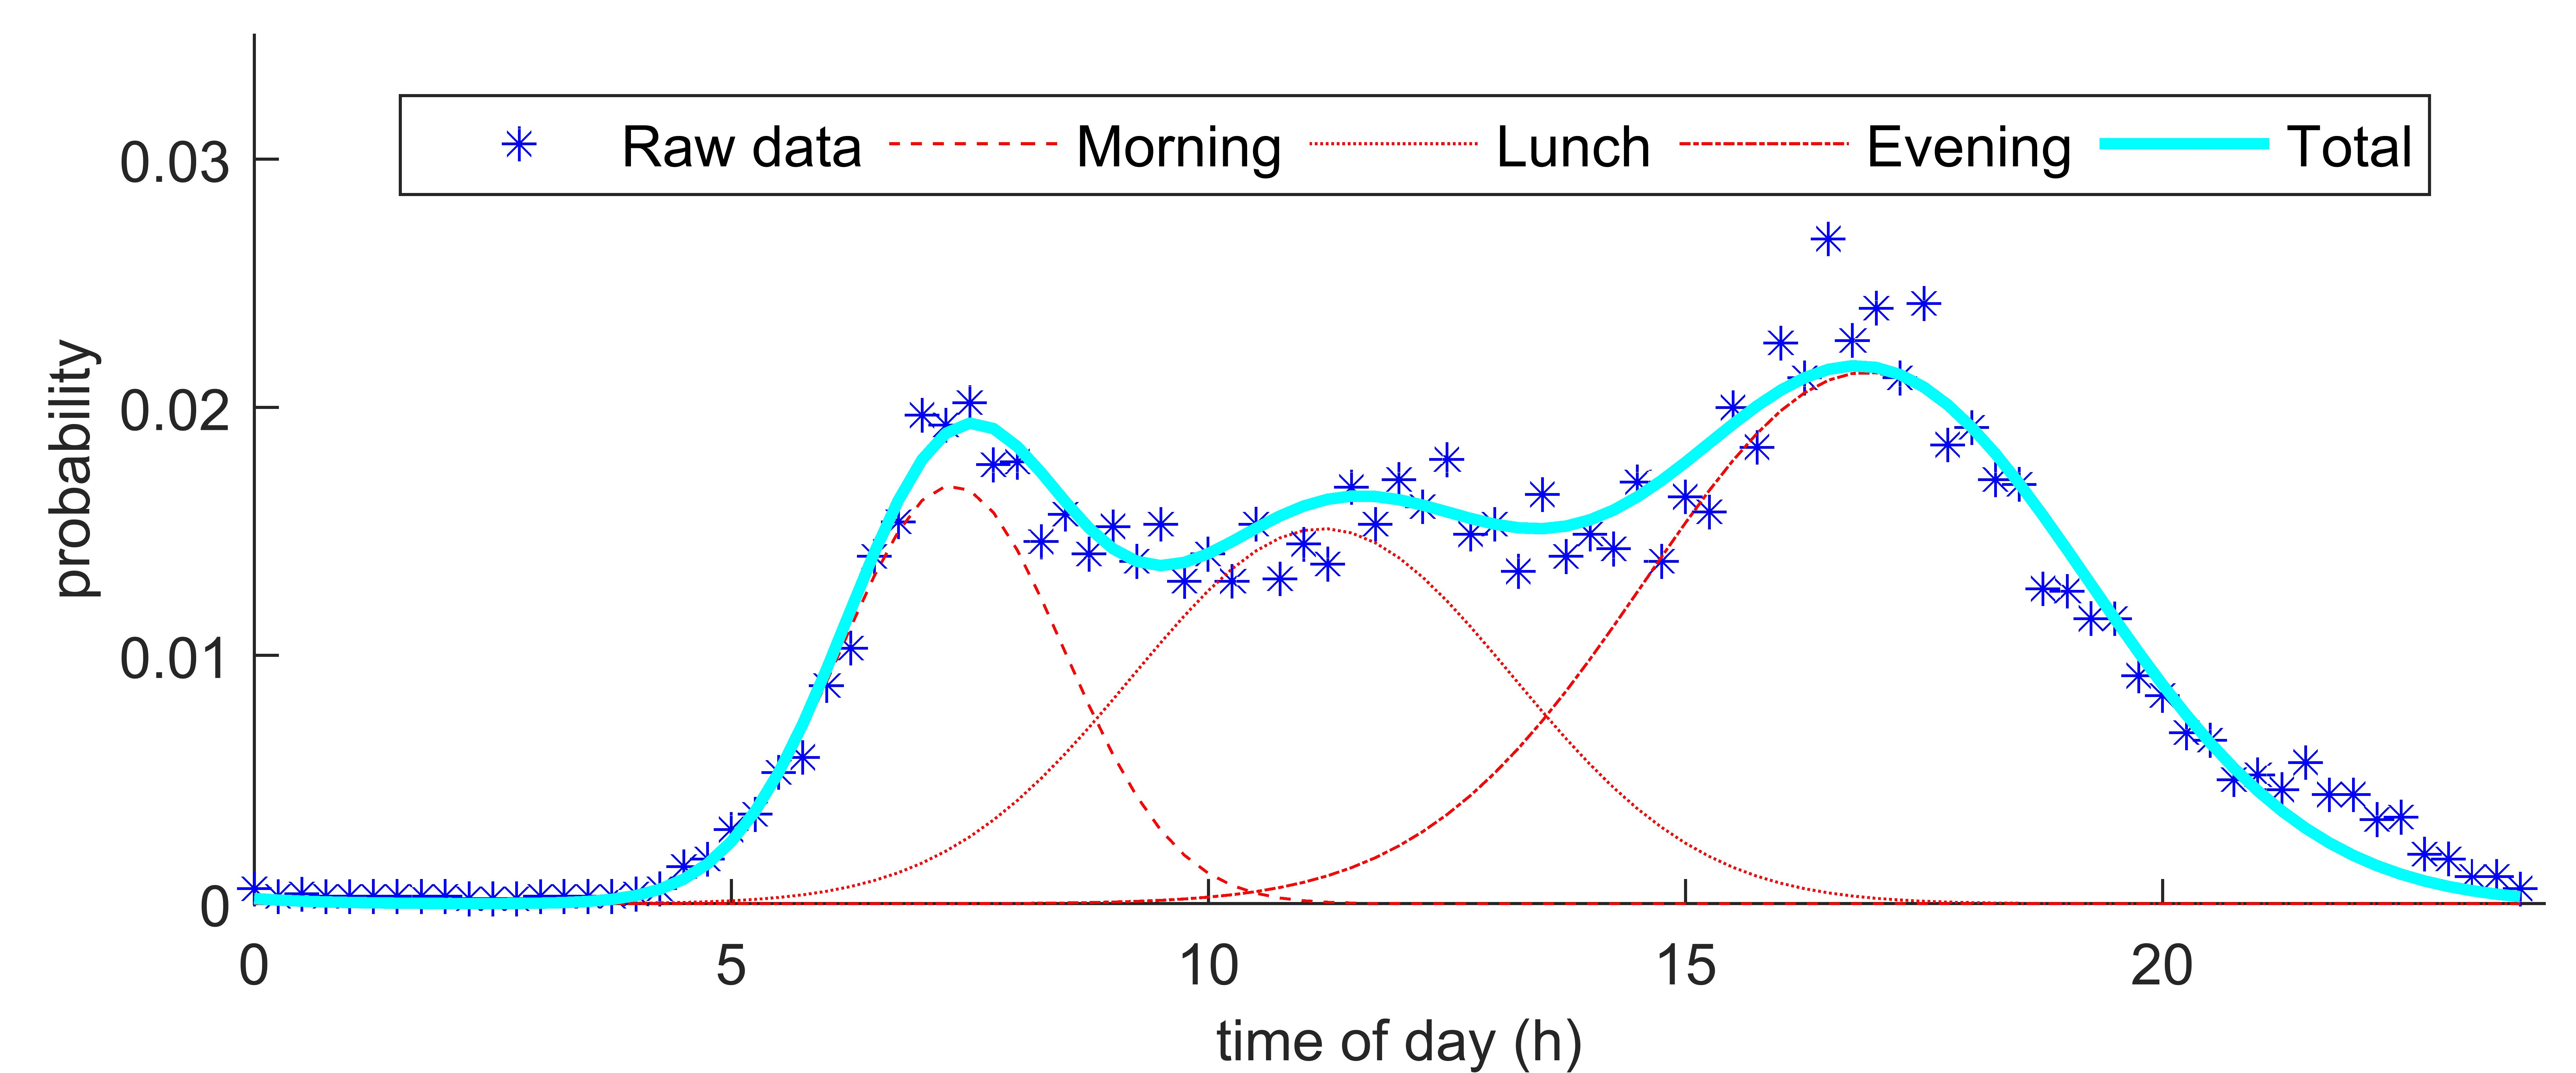
\includegraphics[width=0.8\textwidth]{_chapter4/fig/starting-a-trip-probability}
	\caption{The probability of starting a trip at a particular time during a weekday, extrapolated into three normal distributions (RMS error: $9.482\%$).}
	\label{ch4:fig:starting-a-trip-probability}
\end{figure}


The second statistical data (i.e. the data capturing the probability distribution of a trip being of a certain distance) was also extracted from the dataset and approximated using probability distributions.
This approximation was performed for both the weekdays (i.e. $w_{wd}(d)$) and weekends (i.e. $w_{we}(d)$) data.
The Weibull function was chosen to fit these probability distributions to the original data since it best suited the underlying data distribution - it is defined as follows:

\begin{equation}
\hat{w}_x(\gamma_x,k_x,d) :=
	\begin{cases}
		\frac{k_x}{\gamma_x}\left(\frac{d}{\gamma_x}\right)^{k_x-1}\exp\left[-\left(\frac{d}{\gamma_x}\right)^{k_x}\right] &\text{if } d \geq 0 \\
		0 &\text{if } d < 0
	\end{cases}
	\label{ch4:equ:weibull-distribution}
\end{equation}


Similar to the approximation of the probability of starting a trip, a minimisation problem was designed to fit the two probability distributions to their original data.

\begin{equation}
\begin{split}
	\min_{\gamma, k}& \int \left(\hat{w}_{x}(d) - w_{x}(d)\right)^2 dd\\
	\text{s.t.}& 1 = \int \hat{w}_{x}(d) dd
\end{split}
\label{ch4:equ:trip-distance-minimisation}
\end{equation}

This problem was also solved using the same GRG algorithm and for better readability, $\gamma_x$ and $k_x$ are dropped within the text - i.e. $\hat{\omega}_x(\gamma_x,k_x,d)$ is abbreviated by $\hat{\omega}_x(d)$.
As a result, the weekday trip distance distribution, $\hat{w}_{wd}(d)$, and the weekend trip distribution, $\hat{w}_{we}(d)$, could be estimated.
The computed function parameters for these two estimated distribution functions are tabulated in Table~\ref{ch4:tab:trip-distance-probailility}.
Furthermore, their resulting probability distributions are plotted in comparison to the real data (i.e. $w_{wd}(d)$ and $w_{we}(d)$) in Figure~\ref{ch4:fig:trip-distance-probability}.

\begin{table}\centering 
	\begin{tabular}{ccc}
	\hline
	\textbf{Equation} \boldmath{$\hat{w}_x(d)$} & \boldmath{$\gamma_x$} \textbf{(Scale)} & \boldmath{$k_x$} \textbf{(Shape)} \\
	\hline
	$\hat{w}_{wd}(t)$ & 15.462 & 0.6182 \\
	$\hat{w}_{we}(t)$ & 38.406 & 0.4653\\
	\hline
	\end{tabular}
	\caption{Parameters for Weibull distributions.}
	\label{ch4:tab:trip-distance-probailility}
\end{table}


\begin{figure}\centering
	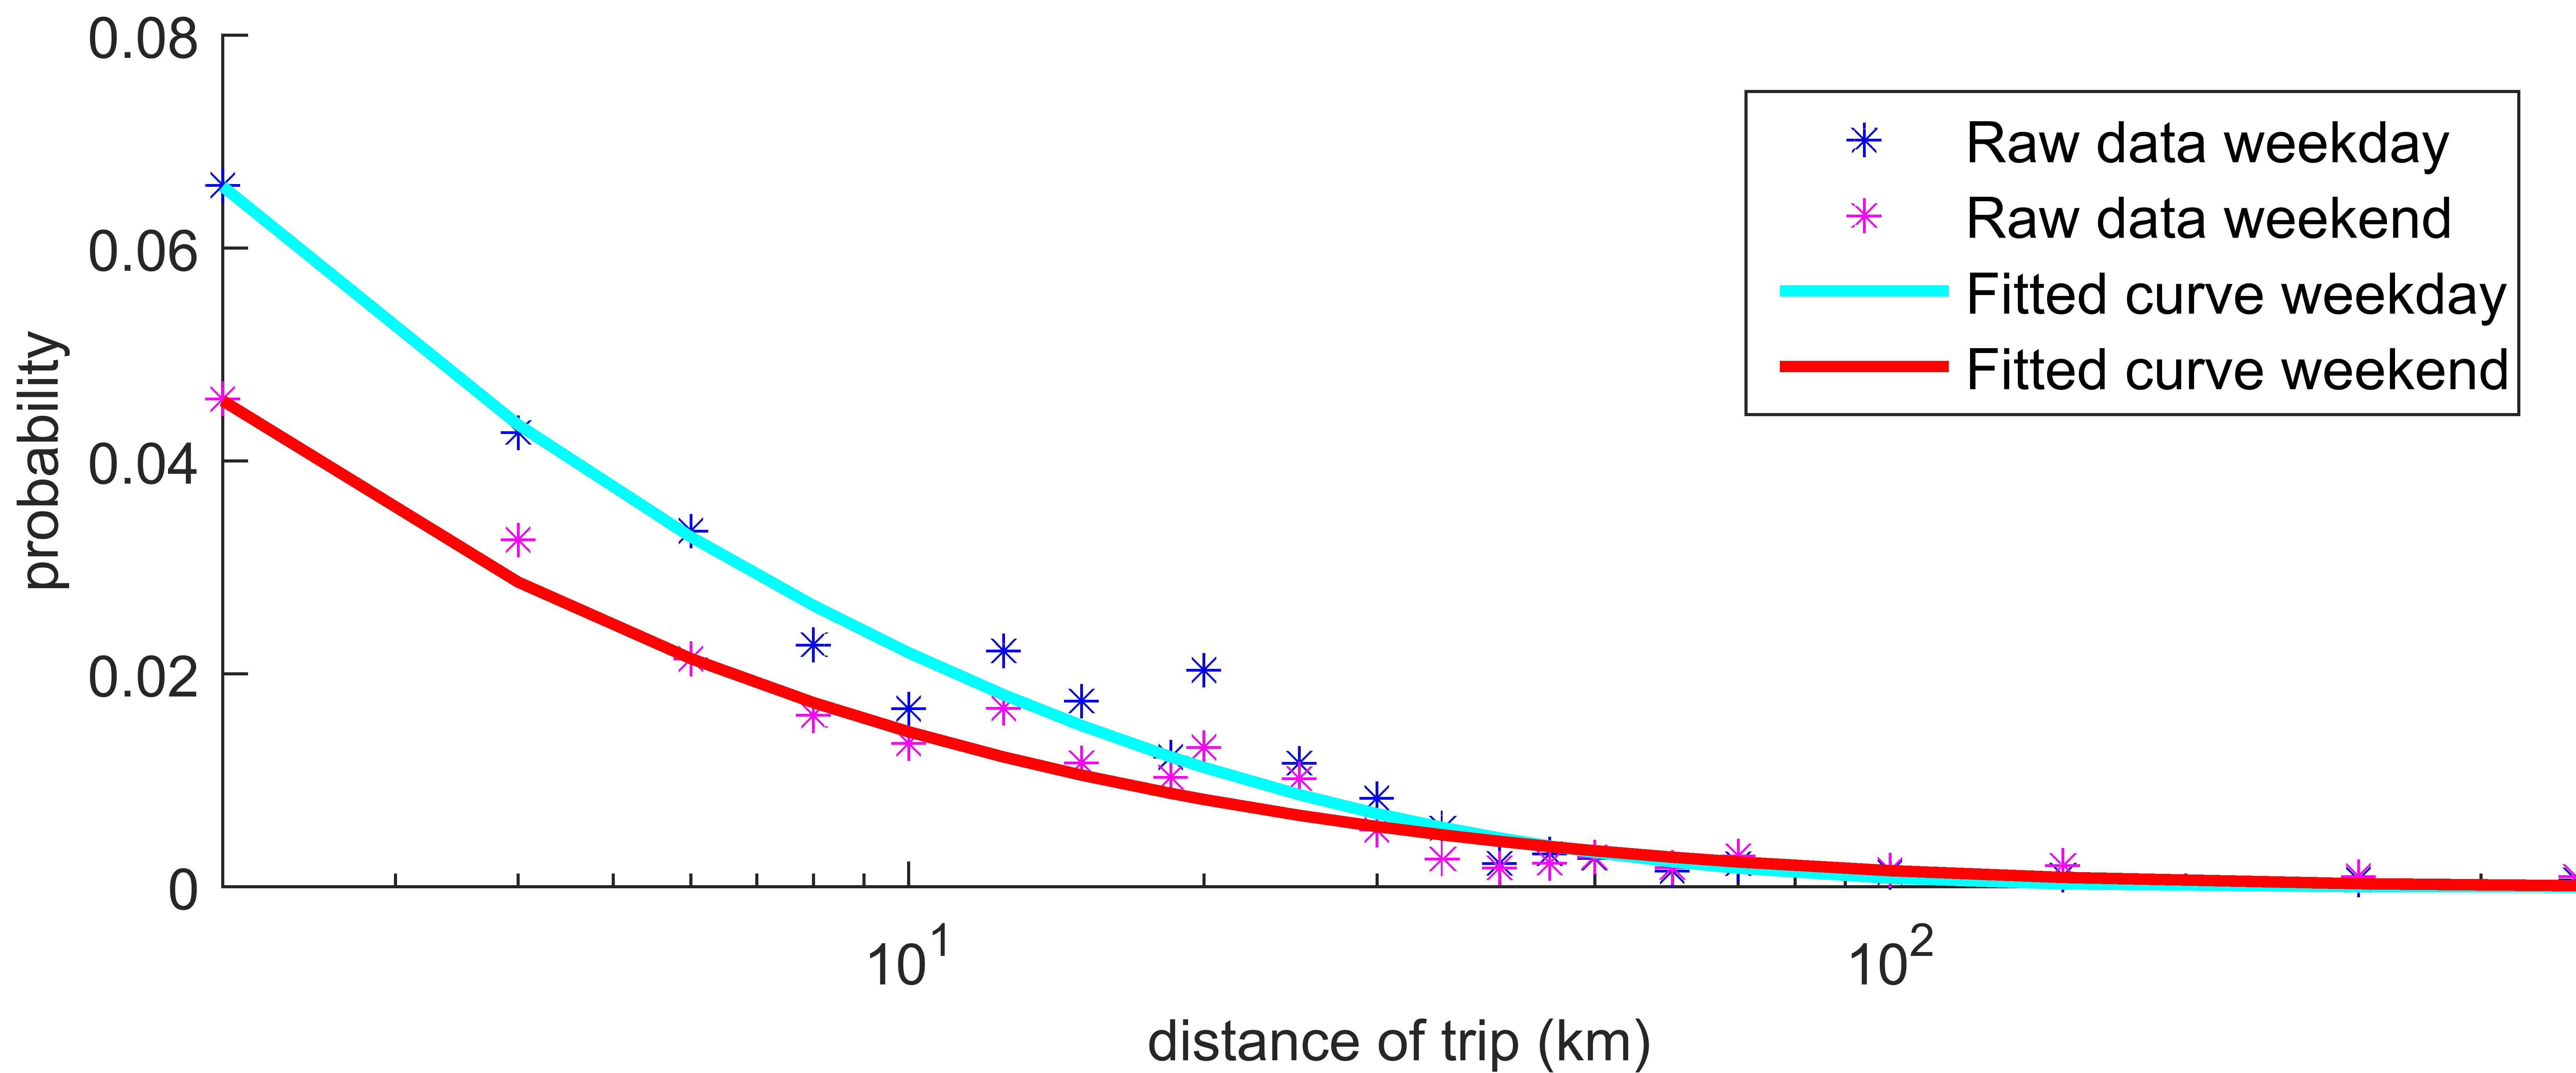
\includegraphics[width=0.8\textwidth]{_chapter4/fig/trip-distance-probability}
	\caption{The probability of a trip being of a particular distance during a weekday, extrapolated into a Weibull distribution (RMS error: $3.791\%$).}
	\label{ch4:fig:trip-distance-probability}
\end{figure}

 
In addition to these probabilities an average driving speed of 56 kmh \hlrem{(}\hladd{ or} 35 mph\hlrem{) and an average driving energy efficiency of 0.1305 kWh/kmh (0.21 kWh/mph) are}\hladd{ is} taken from the \textit{UK Government Digital Service} dataset \cite{UKGovernmentDigitalService2013}\hladd{ and an average driving energy consumption of 0.1305 kWh/km or 0.21 kWh per mile is used, based on a BMW i3 energy demand measured during its \textit{New European Driving Cycle} (NEDC) }\cite{BMW_press_i3}.
Using the predicted driving distance and\hlrem{ average driving speed with the} driving energy efficiency, it is possible to estimate an EV's energy demand upon arrival.
A single EV charging profile is then estimated by starting to charge from the EV's predicted arrival time until the energy demand has been met.
To do so a maximum charging power of the UK's average household circuit rating (i.e. 7.4kW) and an immediate disconnection of the EV upon charge completion were assumed to comply with the guidance of the UK's \textit{Electric Vehicle Home Charging Scheme} \cite{EVHomeCharging}.
\hladd{It is worth mentioning, that a more homogeneous energy demand may be estimated when using different polynomial efficiency functions.
However, to provice a general estimate of charging demand, using the data from a field tested vehicle is assumed sufficient for the work presented here.}

\begin{figure}\centering
 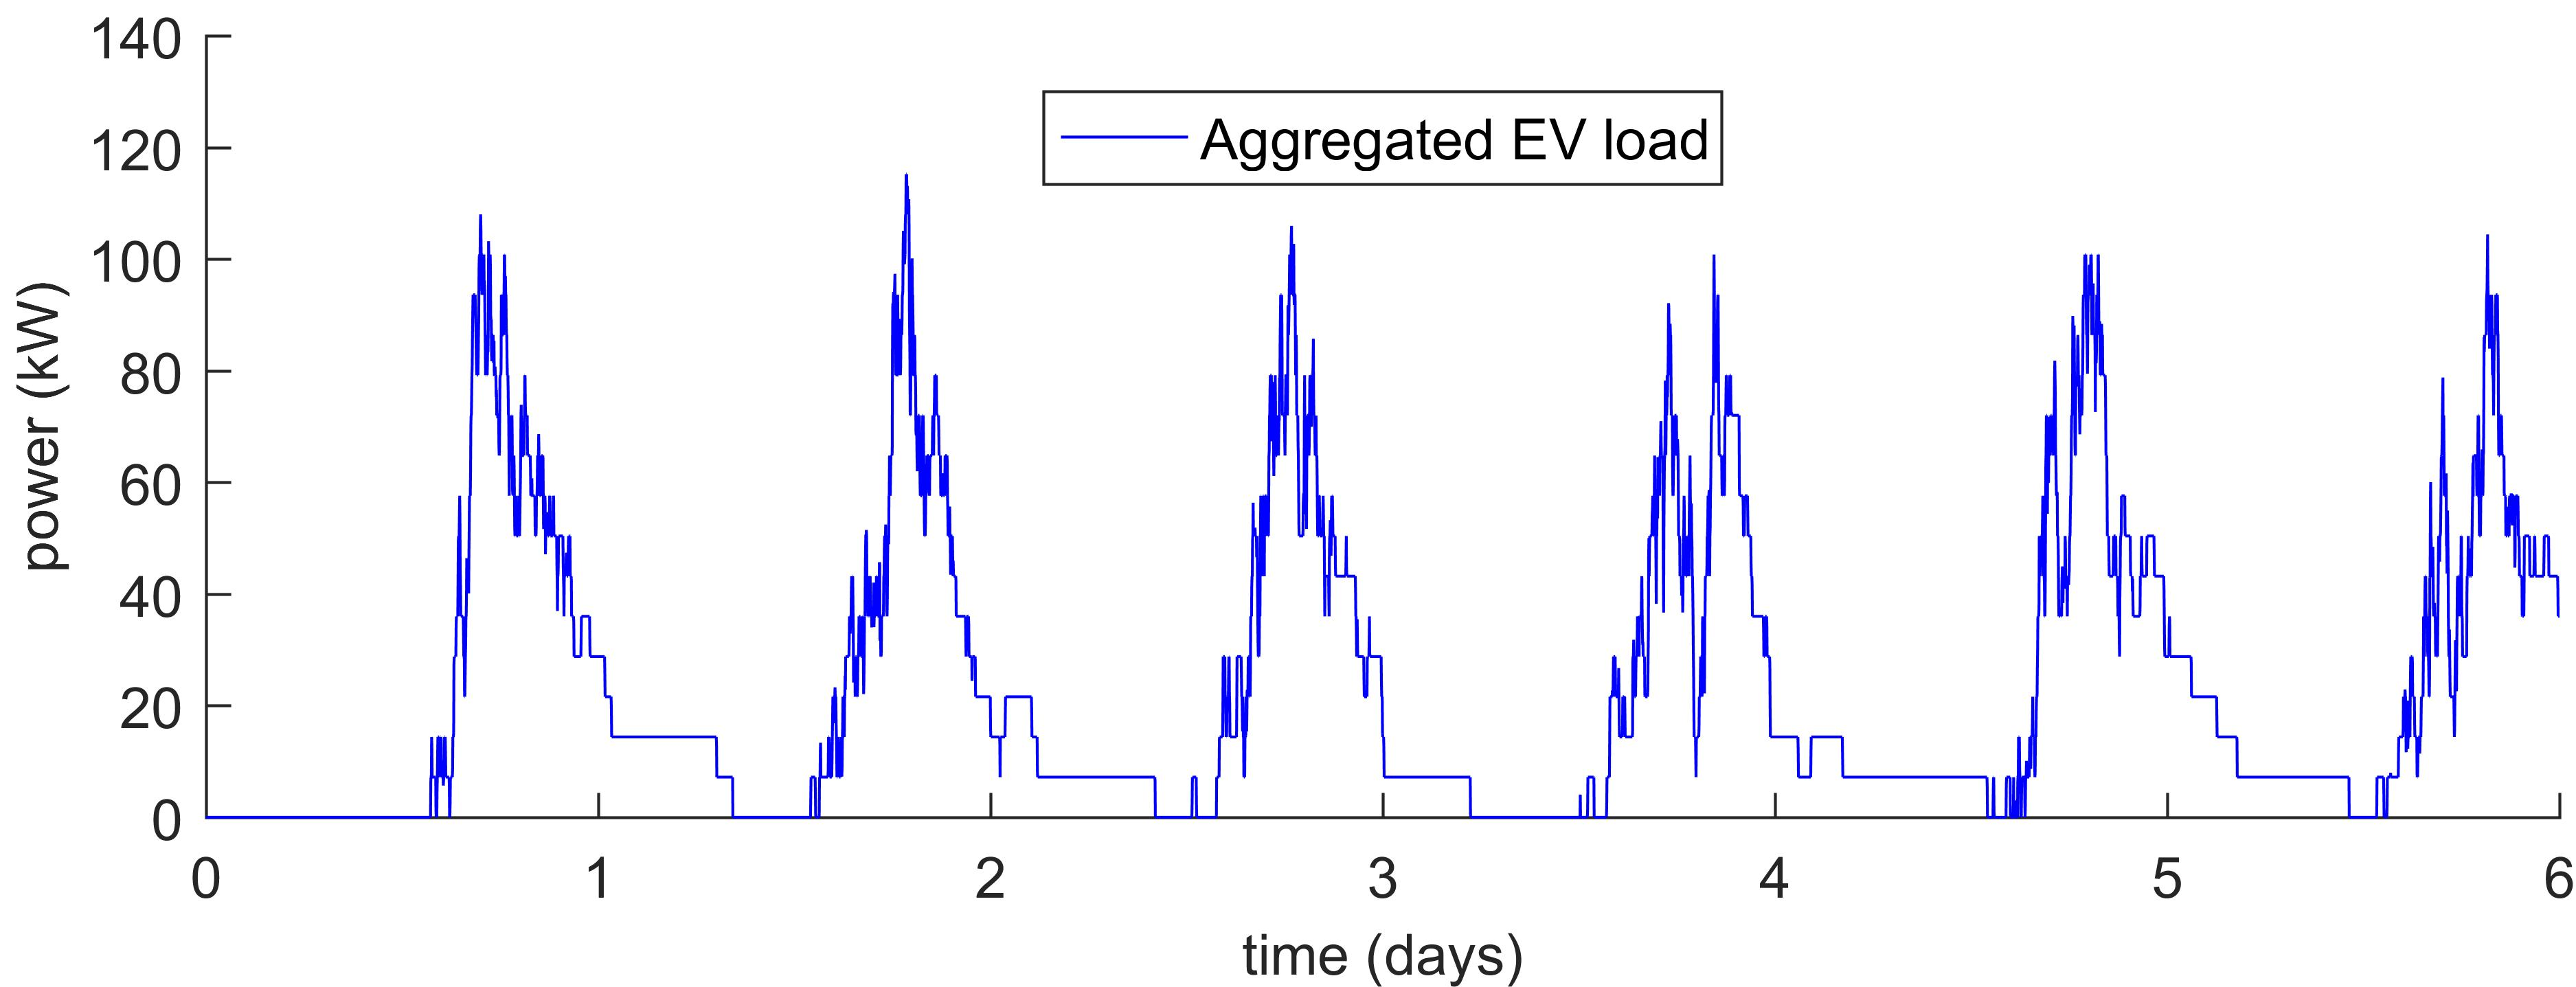
\includegraphics[width=0.8\textwidth]{_chapter4/fig/aggregated-ev-power}
 \caption{Excerpt from the aggregated 50 EVs; charging powers that were each generated from the empirical models.}
 \label{ch4:fig:aggregated-ev-power}
\end{figure}


Generating several of those charging profiles and aggregating them produces an estimated charging demand for an entire fleet of EVs.
To provide an example, charge demand profiles for 50 EVs were generated, aggregated and plotted in Figure~\ref{ch4:fig:aggregated-ev-power}.
This plot shows the expected magnitude and variability in energy demand that is required to charge several EVs at consumers' homes based on the vehicles' daily usage.

This model's EV charging behaviour has been implemented to reflect EV demand if applied today without widespread smart charging infrastructure.
It does therefore reflect the worst assumable charging scenario.
This model's data is used to simulate additional demand in the power network which is supported by batteries whose model is detailed in the next section.

\subsection{Battery Modelling}

In this chapter a similar BESS model is used as the one that has already been introduced in Chapter~\ref{ch1} and in Chapter~\ref{ch2} of this thesis (i.e. see Section~\ref{ch1:subsec:battery-model} and Section~\ref{ch2:subsec:esmu-model}).
The following paragraphs are however used as a reminder of this model for convenience.
In summary, the battery model consists of a self-discharge loss (i.e. $\mu$ where $\mu \in (0, 1]$) that is dependent on the current State Of Charge (SOC) and the model contains an energy conversion efficiency (i.e. $\eta$ where $\eta \in (0, 1]$) to compute the amount of energy that is lost when charging or discharging this battery.

\nomenclature[L]{$p_\text{bat}(t)$}{Battery power at time $t$, where $p_\text{bat}(t) \in \mathbb{R}$}
\nomenclature[L]{$\text{SOC}(t)$}{Battery state of charge at time $t$, where $\text{SOC}(t) \in [0, 1]$}
\nomenclature[L]{$\Delta\text{SOC}(t)$}{Change in SOC during time period $\Delta t$, where $\Delta\text{SOC}(t) \in [-1, 1]$}
\nomenclature[L]{$\mu$}{Self-discharge loss factor, where $\mu \in (0, 1]$}
\nomenclature[L]{$\eta$}{Energy conversion efficiency, where $\eta \in (0, 1]$}
\nomenclature[L]{$\hat{\eta}$}{Direction dependent energy conversion efficiency, where $\hat{\eta} \in (0, 1]$}
\nomenclature[L]{$\text{SOC}_\text{min}$}{Minimum rated SOC for limited battery operation, where $\text{SOC}_\text{min} < \text{SOC}_\text{max}$ and $\text{SOC}_\text{min} \in [0, 1]$}
\nomenclature[L]{$\text{SOC}_\text{max}$}{Maximum rated SOC for limited battery operation, where $\text{SOC}_\text{min} < \text{SOC}_\text{max}$ and $\text{SOC}_\text{max} \in [0, 1]$}
\nomenclature[L]{$C$}{Battery capacity, where $C \in \mathbb{R}_{>0}$}
\nomenclature[L]{$P_\text{max}$}{Power rating of battery, where $P_\text{max} \in \mathbb{R}_{>0}$}
\nomenclature[L]{$\Delta t$}{Sampling period, where $\Delta t \in \mathbb{Z}_{>0}$}

In an ideal battery the change in SOC is determined by the battery power $p_\text{bat}(t)$.
By sampling battery operation at a regular period (i.e. $\Delta t$) the energy transferred into the battery can be described as $p_\text{bat}(t)\Delta t$.
The change in SOC for this ideal battery that is of capacity $C$ is therefore defined as:

\begin{equation}
\Delta \text{SOC}(t) := \frac{p_\text{bat}(t)\Delta t}{C} = \text{SOC}(t) - \text{SOC}(t-\Delta t)
\label{ch4:equ:change-soc}
\end{equation}


Next, the self-discharge loss is determined by $\mu$ and is included in this ideal battery model to represent the continual loss of energy in the battery - which is typical for chemical energy storage.
This loss, $\Delta\text{SOC}_\text{self-discharge}$, is defined as a proportion of the most recent SOC and is determined using the self-discharge loss factor (i.e. $\mu$) as follows:

\begin{equation}
	\Delta\text{SOC}_\text{self-discharge}(t) := \mu\text{SOC}(t)
	\label{ch4:equ:self-discharge-loss}
\end{equation}


Additionally, to represent the losses in the power electronics and energy conversion process, an energy conversion loss (i.e. $\Delta\text{SOC}_\text{conversion}(t)$) is defined next.
This loss is proportional to the rate at which the battery's SOC changes.
Since a difference is made between charging and discharging BESS, a ``direction dependent energy conversion efficiency'' (i.e. $\hat{\eta}$) is derived from $\eta$ and used as follows:

\begin{equation}
	\Delta\text{SOC}_\text{conversion}(t) := \hat{\eta}\Delta\text{SOC}(t) \text{ where } \hat{\eta} \in (0, 1]
	\label{ch4:equ:conversion-loss}
\end{equation}


Here, the conversion losses in the power electronics are reflected as an asymmetric efficiency that depends on the direction of the flow of energy.
This is done by charging the battery at a lower power when consuming energy and discharging it more quickly when releasing energy.
Mathematically, this is represented as:

\begin{equation}
\hat{\eta} =
	\begin{cases}
		\eta &\text{if } \Delta\text{SOC}(t) \geq 0 \\
		\frac{1}{\eta} &\text{if } \Delta\text{SOC}(t) < 0
	\end{cases}
\label{ch4:equ:energy-conversion-adjustment}
\end{equation}


When substituting the self-discharge loss from Equation~\ref{ch4:equ:self-discharge-loss} (i.e. $\Delta\text{SOC}_\text{self-discharge}$) and conversion losses from Equation~\ref{ch4:equ:conversion-loss} (i.e. $\Delta\text{SOC}_\text{conversion}$) into the SOC evolution equation, then the full battery model (i.e. the transition from $\text{SOC}(t)$ to $\text{SOC}(t+\Delta t)$) can be derived as follows:

\begin{equation}
	\begin{split}
		\text{SOC}(t+\Delta t) :&= \Delta\text{SOC}(t) - \Delta\text{SOC}_\text{self-discharge}(t) - \Delta\text{SOC}_\text{conversion}(t)\\
		&= (1-\mu)\Delta\text{SOC}(t) - \hat{\eta}\Delta\text{SOC}(t)	
	\end{split}
	\label{ch4:equ:soc-transition}
\end{equation}


In addition, both the SOC and the battery power (i.e. $p_\text{bat}(t)$) are constrained due to the device's maximum and minimum energy storage capabilities (i.e. respectively $\text{SOC}_\text{max}$ and $\text{SOC}_\text{min}$ and maximum charge and discharge rate $P_\text{max}$).
These limitations are captured in Equations~\ref{ch4:equ:soc-range} and Equation~\ref{ch4:equ:charge-discharge-range}, respectively.

\begin{equation}
\text{SOC}_\text{min} \leq \text{SOC}(t) \leq \text{SOC}_\text{max}
\label{ch4:equ:soc-range}
\end{equation}


\begin{equation}
\left|p_\text{bat}(t)(t)\right| \leq \text{P}_\text{max}
\label{ch4:equ:charge-discharge-range}
\end{equation}


\subsection{Network Models}
\label{ch4:subsec:network-models}

Similar to Chapter~\ref{ch1} of this thesis, the Open Distribution System Simulator (OpenDSS) that is developed by the Electronic Power Research Institute (EPRI) was used in order to simulate the LV energy distribution networks.
It requires element-based network models including line, load and transformer information to generate realistic power flow results.

\begin{figure}\centering
	\subfloat[]{%
		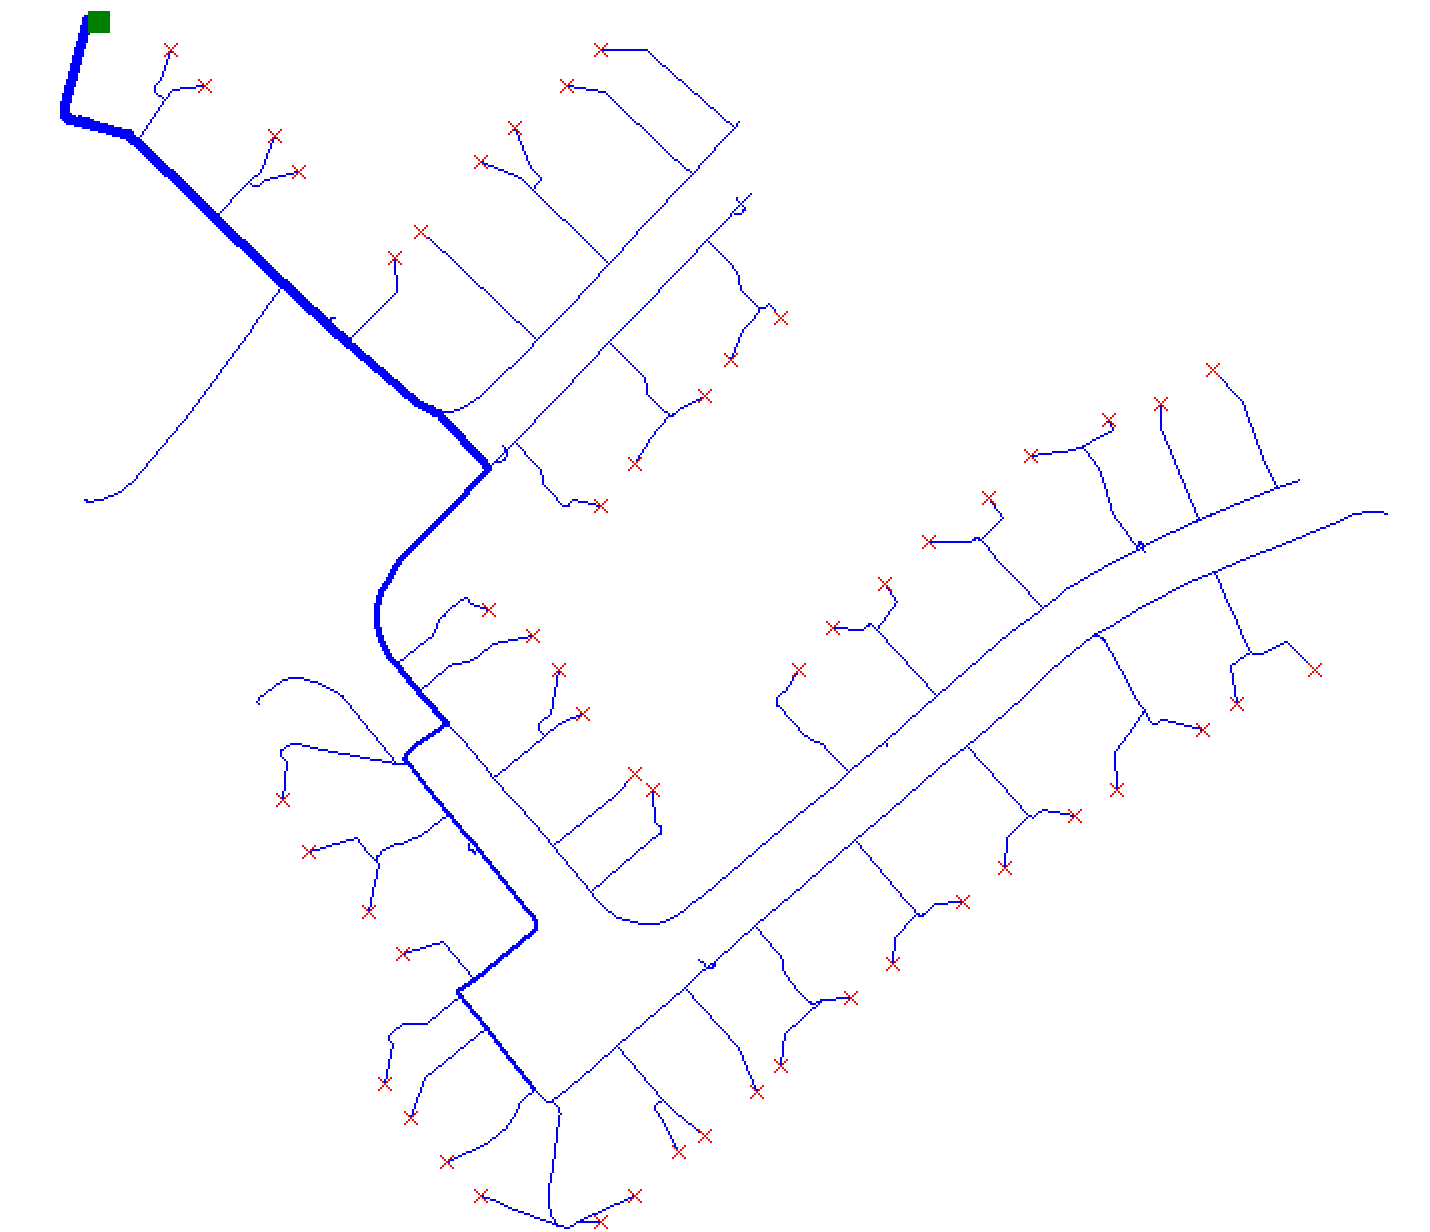
\includegraphics[width=0.5\linewidth]{_chapter4/fig/network-EULVFeeder}%
		\label{ch4:subfig:network-ieee}%
	}
	\subfloat[]{%
		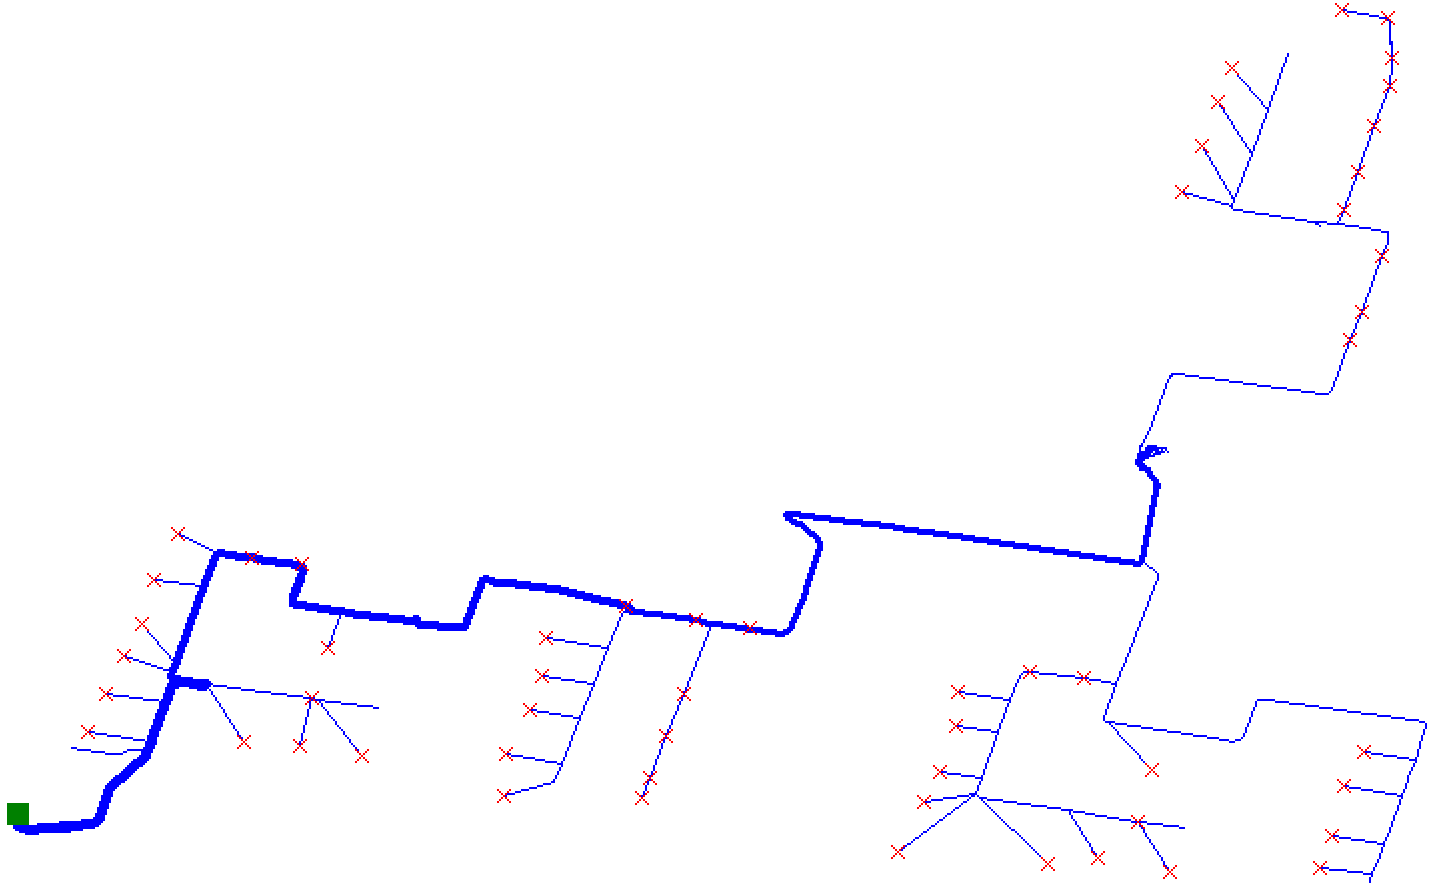
\includegraphics[width=0.5\linewidth]{_chapter4/fig/network-Deepdale_FD01}%
		\label{ch4:subfig:network-ssen}%
	}
	\caption{Sample OpenDSS power networks, where consumers are indicated as red crosses and 11/0.416-kV substations are marked with a green square. Here, (a) is the IEEE PES EU LV test feeder, and (b) is a SSEN Common Information Model (CIM) based feeder}
	\label{ch4:fig:network}
\end{figure}


Initial simulations were conducted using the IEEE's European Low Voltage Test Feeder \cite{EULVFeeder2015} and later six detailed UK feeder models were added that are based on real power distribution networks.
These models were provided by the project partner Scottish and Southern Electricity Networks (SSEN).
The SSEN circuit models were provided as Common Information Models (CIM) during the collaboration on the New Thames Valley Vision (NTVV) project \cite{NTVV2016}.
An example of the IEEE EU LV Test feeder and a UK feeder provided by SSEN are shown in Figure~\ref{ch4:subfig:network-ssen} and Figure~\ref{ch4:subfig:network-ssen}, respectively.
A summary of all model's parameters is given in the Table~\ref{ch4:tab:model-parameters}.

\begin{table}\centering
\begin{tabular}{r | c | c c c c c c}
%\multirow{2}{*}{\textbf{Parameter}} & \textbf{IEEE EU} & \multicolumn{6}{c}{\multirow{2}{*}{\textbf{SSEN LV Feeders}}}\\
% & \textbf{LV Test Feeder} & \\
Parameter & IEEE Feeder & \multicolumn{6}{c}{SSEN Feeders}\\
\hline
network No. & 1 & 2 & 3 & 4 & 5 & 6 & 7\\
\hline
no. of customers & 55 & 56 & 53 & 91 & 59 & 88 & 37\\
mean customer load (VA) & 227 & 227 & 231 & 241 & 224 & 237 & 237\\
max. customer load (kVA)& 16.8 & 16.8 & 16.8 & 19.5 & 16.8 & 19.5 & 16.8\\
mean net. load (kVA)& 24.4 & 24.9 & 23.9 & 41.9 & 25.6 & 38.9 & 16.3\\
max. net. load (kVA)& 72.6 & 72.7 & 72.2 & 92.9 & 73.5 & 89.6 & 60.5\\ 
%\hline
%Customer connection & Single-phase & \multicolumn{6}{c}{Single-phase}\\
%\hline
%\multirow{2}{*}{Feeder line model} & Three-phase & \multicolumn{6}{c}{Three-phase}\\
% & implicit-neutral & \multicolumn{6}{c}{explicit-neutral}\\
\end{tabular}
\caption{Network model parameters.}
\label{ch4:tab:model-parameters}
\begin{tabular}{ccc}
%\multicolumn{1}{c}{\footnotesize $^1$ These networks are shown in Figure~\ref{ch4:fig:network}.}
\end{tabular}
\end{table}

Throughout the remainder of this chapter, all excerpt and time series results were extracted from experiments with the IEEE EU LV Test feeder (i.e. Network No. 1).
Any further results are then based on an aggregation of all networks to include their network diversity in the analysis.

The same model-derived EV data and the IEEE provided consumer demand profiles were used in all power flow simulations.
The resulting demand profiles therefore represent the total daily electricity demand of households with connected EVs.
These profiles were sampled at $\Delta t = 1\text{ minute}$.
The OpenDSS simulation environment was controlled using MATLAB that communicated with OpenDSS through its Common Object Model (COM) interface which is accessible using Microsoft's ActiveX server bridge.
